\documentclass[11pt]{jsarticle}
\usepackage{amsmath}
\usepackage{color}
\usepackage[dvipdfmx]{graphicx}
% https://qiita.com/BitPositive/items/6b13e2038d628c33be8e latexのインストールと使い方
\begin{document}


\title{{\normalsize FRA-SA-2020-ABCWG01-02}\\
  再生産関係の推定・管理基準値計算・将来予測シミュレーションに関する技術ノート \\
  \Large (令和2年度研究機関会議版)
}
\author{ABCWG}
\date{\today}
\maketitle

\section{平成31年度版からの変更点}
\begin{itemize}
\item 自己相関係数推定における同時推定と2段階推定の選択に関して追記
\item 簡易MSEに関する記述を追加(\ref{sec:mse}節)  
\item 過去にさかのぼってHCRを適用した場合のシミュレーションについてを追加(\ref{sec:whatif}節)
\end{itemize}

\section{基本的な式と記号の説明}
本資料で使われる主要な数式記号の定義(表\ref{table_definition}),ホッケー・スティック(HS)\cite{hockey},ベバートン・ホルト(BH)\cite{beverton},リッカー(RI)\cite{ricker}型の再生産関係式,個体群動態の基本的な式を以下に示した. 

\subsubsection*{ホッケー・スティック型再生産関係(HS)}
\begin{equation}
  \mathrm{R}(S\!B_{t}|a,b)=\begin{cases}
    a  S\!B_{t-S_{\mathrm{min}}} & (S\!B_{t-S_{\mathrm{min}}} < b) \\
    a  b                 & (S\!B_{t-S_{\mathrm{min}}} \geq b)
  \end{cases}
  \label{HS}
\end{equation}
ただし,親魚量と加入量が線形関係の場合には過去最大親魚量をHSの折れ点と仮定する.一方,観察された親魚量の範囲で加入がほぼ一定となる場合には,HSの折れ点を過去最小親魚量とする.

\subsubsection*{ベバートン・ホルト型再生産関係(BH)}
\begin{eqnarray}
  \mathrm{R}(S\!B_{t}|a,b)=\frac{a S\!B_{t-S_{\mathrm{min}}}}{1 + b S\!B_{t-S_{\mathrm{min}}}}
  \label{BH1}
\end{eqnarray}
%または  % 今回の会議用バージョンということで,この式の定義はもう載せない
%\begin{eqnarray}
%  \hat{N}_{t,S_{\mathrm{min}}}=\frac{a S\!B_{t-S_{\mathrm{min}}}}{1 + \frac{S\!B_{t-S_{\mathrm{min}}}}{b}}
%  \label{BH2}
%\end{eqnarray}

\subsubsection*{リッカー型再生産関係(RI)}
\begin{eqnarray}
  \mathrm{R}(S\!B_{t}|a,b) = a S\!B_{t-S_{\mathrm{min}}}   \exp{(-b S\!B_{t-S_{\mathrm{min}}})}
  \label{RI1}
\end{eqnarray}
%または
%\begin{eqnarray}
%  \hat{N}_{t,S_{\mathrm{min}}}= a S\!B_{t-S_{\mathrm{min}}}   \exp{(-\frac{S\!B_{t-S_{\mathrm{min}}}}{b})}
%  \label{RI2}
%\end{eqnarray}

%式\ref{BH2},\ref{RI2}はパラメータbがHSのときのパラメータbと同じ単位を持つため,BH,RIの当てはめにおいては,今後は式\ref{BH2},\ref{RI2}の使用が好ましい.

\subsubsection*{個体群動態の式}
個体群動態の決定論的な基本式は以下のような年齢構造モデルで表す.
\begin{equation}
  N_{s,t} = \begin{cases}
    \mathrm{R}(S\!B_{t}|a,b)  &     s = S_\mathrm{min} \\    
    N_{s-1, t-1}  \exp(-M_{s-1,t-1}-F_{s-1,t-1} )  &    S_\mathrm{min} < s < S_\mathrm{max} \\
    N_{s-1, t-1}  \exp(-M_{s-1,t-1}-F_{s-1,t-1} ) + N_{s, t-1}  \exp(-M_{s,t-1}-F_{s,t-1}) &   s=S_{\mathrm{max}}
  \end{cases}
  \label{future_eq}
\end{equation}

\section{再生産関係式のパラメータ推定\label{SRest}} 
まず,残差の自己相関を考慮せずにパラメータ$a$,$b$を推定する(\ref{estab}節).このときは最小二乗法または最小絶対値法を使用する.さらに,残差の自己相関も考慮するかどうかを検討する。
\subsection{パラメータ$a$,$b$の推定\label{estab}}
観測値と再生産関係式からの予測値との残差 $\varepsilon_t \, (T_1 \leq t \leq T_2)$を
\begin{eqnarray}
  \varepsilon_t = \log (N_{S_{\mathrm{min}},t}^{\mathrm{obs}}) - \log \mathrm{R}(S\!B_{t-S_{\mathrm{min}}}^{-mathrm{obs}}|a,b)
\end{eqnarray}
と定義し,最小二乗法の場合には
\begin{eqnarray}
  \sum_{t=T_1}^{T_2} \varepsilon_t^2
\end{eqnarray}
最小絶対値法の場合には
\begin{eqnarray}
  \sum_{t=T_1}^{T_2} | \varepsilon_t |
\end{eqnarray}
を最小化することで,パラメータ$a$,$b$を推定する.最小絶対値法の方が,外れ値の影響を受けにくく,頑健な推定値が得られやすい.AIC等の情報量規準で使用される対数尤度は,最小二乗法の場合は正規分布,最小絶対値法の場合はラプラス分布を用いて計算される.どちらの最適化法を用いた場合でも,残差の標準偏差$\sigma$は
\begin{eqnarray}
  \sigma = \sqrt{\frac{1}{n} \sum_{t=T_1}^{T_2} \varepsilon_t^2}
\end{eqnarray}
と定義する.

\subsection{残差の自己相関の有無を判断する\label{estrho}}
推定された再生産パラメータ$a$,$b$のもとで,加入の予測値に対する観測値の残差$\varepsilon_t$に自己相関があるかどうかを検討する.自己相関を導入したほうがよいかどうかは,$\rho$が統計的に有意かどうかやAIC等を用いて判断する.また,簡便にはR\cite{R}で実装されている関数\verb|acf|で出力される図で示される95\%信頼区間等からも判断できる.

自己相関を推定する方法としては,再生産関係式のパラメータ$a$,$b$を推定してから,残差についての自己回帰モデル(式\ref{rho_eq})で自己相関係数$\rho$を推定する二段階の手法(二段階推定)が簡便である。
\begin{eqnarray}
  \varepsilon_t = \rho \varepsilon_{t-1} + \xi_t
  \label{rho_eq}
\end{eqnarray}
ここで $\xi_t$は
\begin{eqnarray}
  \xi_t \sim \mathrm{Normal}(0, (1-\rho^2) \sigma^2)) 
\end{eqnarray}
\begin{eqnarray}
  \sigma= \sqrt{ \frac{1}{n} \left[ \varepsilon_{T_1}^2 + \frac{1}{1-\rho^2} \sum_{t=T_1+1}^{T_2} (\varepsilon_t-\rho \varepsilon_{t-1})^2 \right]}
\end{eqnarray}
二段階推定は安定的なパラメータ推定が得られる場合が多い.

一方、$a$,$b$,$\rho$を含む正確尤度 (exact likelihood, 式\cite{subsec:rho})を最小化することで,$a$,$b$,$\rho$を同時に推定する方法(同時推定)もある。同時推定によるパラメータ推定は,最尤推定値を得ることが難しい,推定値にバイアスが生じる,推定値が不安定になるなどの問題点が指摘されている\cite{johnson}.特に,HSを用いた時に局所解が複数存在し,推定値がさらに不安定になる現象も確認されている(未発表)。

$\rho$の推定手法として2段階推定を使うか、同時推定を使うかは、パラメータの安定性や局所解の存在、ブートストラップ等、一連のモデル診断を通じて判断する。ただし、マアジ太平洋系群を模したシミュレーションの結果では、自己相関係数が非常に大きい場合、二段階推定は真の自己相関係数を過小推定する傾向が見られた(\cite{rho_simulation})。そのため、自己相関が非常に大きいと思われ、それが加入変動に大きく影響を与える可能性がある場合、同時推定を用いたほうが加入変動の不確実性をより正確に捉えられると考えられる。ただし、その場合でも、推定パラメータの安定性を十分確認したり、MSEなどを用いて誤りに対する影響を評価する必要はある。

自己相関の影響を除いたときの加入の残差の分散は$(1-\rho^2) \sigma^2$で,自己相関でも説明しきれなかったランダムな加入変動の大きさを示す.平成31年度研究機関会議でSDとして示されている数値は$\sqrt{(1-\rho^2) \sigma^2}$に対応する.

\section{管理基準値の推定}
管理基準値は,推定された再生産関係パラメータと確率的な加入変動等のもとで,漁獲係数を一定にした場合の確率的な平衡状態(時系列的に平均値が一定)となるときの漁獲量や資源量の平均値などを使って推定する.通常は,近年の代表的な年齢別漁獲係数$F_{\mathrm{current},s}$に対して,選択率を保ったまま一律に漁獲圧を削減または増加させるような漁獲係数一定のシナリオを想定する.この場合の将来の漁獲係数は$F_{\mathrm{current},s}$に特定の乗数$\alpha$を乗じた$\alpha F_{\mathrm{current},s}$となる.ここで$1-\alpha$は,例えば$\alpha<1$の場合,目的とする管理基準値を得るために削減すべき漁獲努力量の削減率と解釈される.年齢別漁獲係数$F_{\mathrm{current},s}$は,通常,資源評価最終年を含む直近$l$年分の年齢別漁獲係数の平均値が用いられ,以下のように計算される.
\begin{eqnarray}
  F_{\mathrm{current},s} = \sum_{t=T_3-l+1}^{T_3}\frac{F_{s,t}}{l}
\end{eqnarray}

確率的シミュレーションにおける加入尾数は,再生産関係式から計算される加入尾数にランダムな誤差$\exp (\varepsilon_t^k)$を乗じたものとして計算される.$\varepsilon_t^k$は,対数正規分布の誤差を仮定する場合には
\begin{equation}
  \varepsilon_t^k \sim \begin{cases}
    \mathrm{Normal} (0,\sigma^2 ) & \rho=0 \\
    \mathrm{Normal} (\rho \varepsilon_{t-1}^k,(1-\rho^2) \sigma^2) & \rho>0
  \end{cases}
  \label{epsilon1}
\end{equation}
となる.また,残差リサンプリングによるシミュレーションを実施する場合には
\begin{eqnarray}
  \varepsilon_t^k \sim (\mathrm{random} \, \mathrm{draw} \, \mathrm{from} \, \varepsilon_{t={T_1,…,T_2}})
  \label{epsilon2}  
\end{eqnarray}
となる.

\begin{figure}[t]
  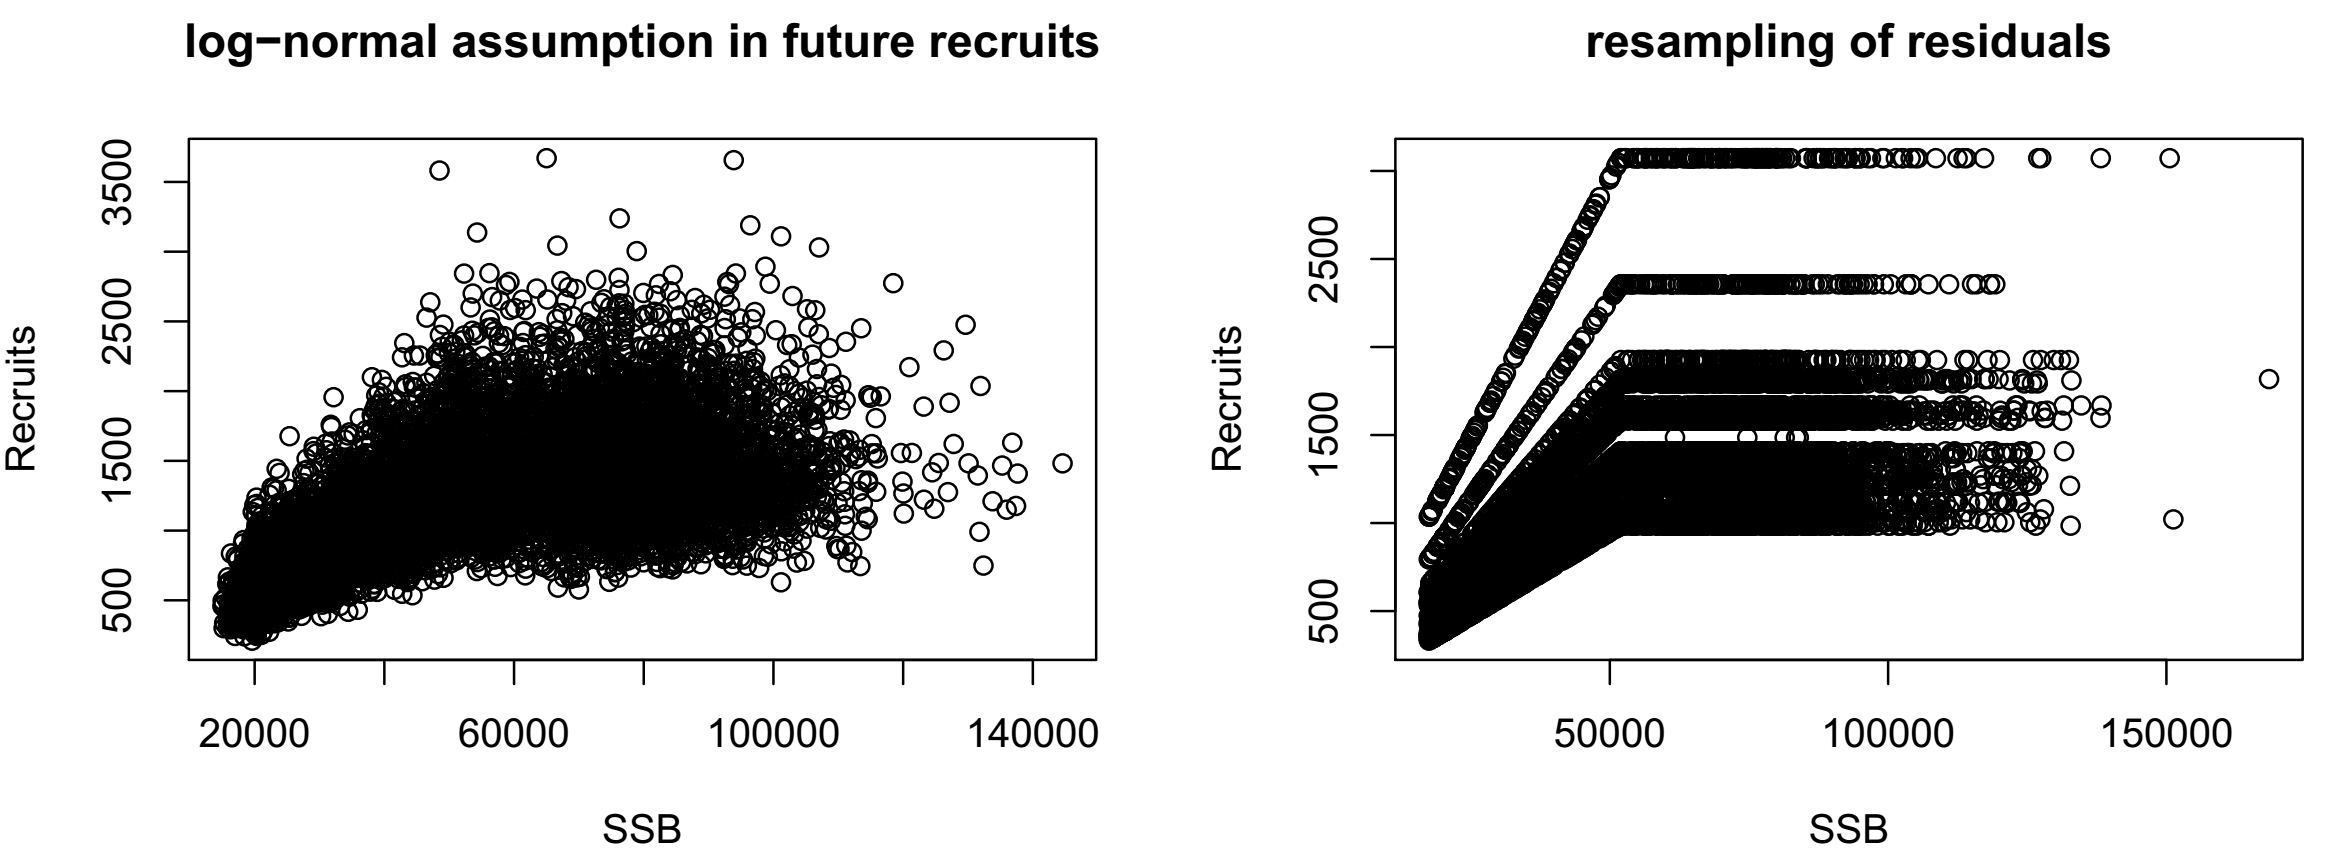
\includegraphics[width=10cm]{fig_resample.png}
  \caption{将来予測における誤差分布の仮定の違い.(左) 対数正規分布の誤差を仮定した場合.(右) 残差のリサンプリングによる誤差を仮定した場合}
  \label{fig_resample}
\end{figure}

以上より,管理基準値計算のために実施する確率的シミュレーションにおける個体群動態式は以下となる.
\begin{equation}
  N_{s,t}^k = \begin{cases}
    \mathrm{R}(S\!B_{t}^k|a,b) \exp (\varepsilon_t^k + \kappa) &     s = S_\mathrm{min} \\    
    N_{s-1, t-1}^k  \exp(-M_{s-1,t-1}-\alpha F_{\mathrm{current},s} )  &    S_\mathrm{min} < s < S_\mathrm{max} \\
    N_{s-1, t-1}^k  \exp(-M_{s-1,t-1}-\alpha F_{\mathrm{current},s} ) + N_{s,t-1}^k  \exp(-M_{s,t-1} - \alpha F_{\mathrm{current},s} ) &   s=S_{\mathrm{max}}
  \end{cases}
  \label{future_eq2}
\end{equation}
ここでは$t \geq T_3$で,$t=T_3$のとき$N_t^k=N_t^{\mathrm{obs}}$,$F_t^k=F_t^{\mathrm{obs}}$とする.$\kappa$は漁獲なしのときの親魚量(初期資源量)$S\!B_0$の決定論的な値(式\ref{future_eq})と,確率的予測値(式\ref{future_eq2})の平均を一致させるためのバイアス補正項で,対数正規分布を仮定する場合には$\kappa=-0.5\sigma^2$,残差リサンプリングをおこなう場合には$-\log( \frac{\sum_{t=T_1}^{T_2} \exp(\varepsilon_t)}{n} )$となる.

管理基準値は,$\alpha$を様々に変え,十分平衡状態に達したと判断される$T_4$年における状態から推定する.経験的には,$T_4=T_3+20G$であれば十分平衡状態に達するようだが,系群によって平衡状態に十分達したと判断される年数を用いる.

\subsection{MSY管理基準値}
MSY管理基準値は,$K$回シミュレーションを実施した場合の$T_4$年における漁獲量$C_{T_4}^k$の平均値($\frac{\sum_{k=1}^K C_{T_4}^k}{K}$)が最大になるような$\alpha$を探索的に求め,推定する.$C_{T_4}^k$は,資源量推定にBaranovの漁獲方程式を使っている場合,
\begin{eqnarray}
  C_{T_4}^k=\sum_{s=S_{\mathrm{min}}}^{S_{\mathrm{max}}} \frac{\alpha F_{\mathrm{current},s}}{\alpha F_{\mathrm{current},s}+M_{s,T_4}}
  \exp(-\alpha F_{\mathrm{current},s}-M_{s,T_4}) N_{s,T_4}^k v_{s,T_4}
\end{eqnarray}
Popeの近似式を使っている場合
\begin{eqnarray}
  C_{T_4}^k=\sum_{s=S_{\mathrm{min}}}^{S_{\mathrm{max}}} (1-\exp(-\alpha F_{\mathrm{current},s})) \exp(-\frac{M_{s,T_4}}{2})N_{s,T_4}^k v_{s,T_4} 
\end{eqnarray}
で計算される.このときの平均漁獲量を$\mathrm{MSY}$, $\alpha F_{\mathrm{current},s}$を$F_{\mathrm{msy},s}$と定義する.また,$F_{s,t}^k=F_{\mathrm{msy},s}$で$K$回シミュレーションを行ったときの$t=T_4$における親魚資源量の平均($\sum_{k=1}^K S\!B_{T_4}^k /K$)が$S\!B_{\mathrm{msy}}$,$\mathrm{MSY}/ \sum_{k=1}^K B_{T_4}^k K^{-1}$をMSYを与える漁獲率($U_{\mathrm{msy}}$)とする.$K$は乱数の違いによって推定値が大きく変わらないくらい十分に大きい数を用いる(自己相関なしの場合は最低2000回,ありの場合は1万回以上が望ましい).

$F_{\mathrm{msy},s}$は年齢別の漁獲係数のベクトルとして与えられ,特定の選択率を前提する.そのため,神戸プロットなどのために,過去に見られた年齢別漁獲係数$F_{t,s}^{\mathrm{obs}}$が$F_{\mathrm{msy},s}$に比べてどの程度大きかった・小さかったか($F/F_{\mathrm{msy}}$)を計算するためには,MSY計算で前提とされた選択率と過去の選択率の違いを考慮する必要がある.具体的には$F_{\mathrm{msy},s}$のときのSPRに一致するような$\alpha F_{t,s}^{\mathrm{obs}}$を求め,$1/\alpha=F/F_{\mathrm{msy}}$と定義する.

\subsection{その他の管理基準値}
その他,平衡状態において特定の平均漁獲量(たとえば,限界管理基準値の標準値となるMSYの60\%や,禁漁水準を与えるMSYの10\%など)や平均親魚量(たとえば$S\!B_0$の30\%など)を達成するような管理基準値を計算する場合も同様に,$t=T_4$において平均漁獲量または親魚量が目的とする値と一致するような$\alpha$を探索的に求め,得られた漁獲係数のもとで平衡状態に達したときの平均親魚量を資源量の管理基準値として用いる.

\section{ABC算定や目標達成確率計算のための将来予測}
漁獲管理規則のもとでの中長期的な将来予測でも,加入誤差については,基本的に式\ref{epsilon1},\ref{epsilon2}などから計算された$\varepsilon_t^k$を用いて計算する.一方,将来の漁獲係数は漁獲管理規則に従って毎年異なる値$F_{s,t}^k$を用いる.したがって,短期予測のための将来予測の個体群動態式は
\begin{equation}
  N_{s,t}^k = \begin{cases}
    \mathrm{R}(S\!B_{t}^k|a,b) \exp (\varepsilon_t^k + \kappa) &     s = S_\mathrm{min} \\    
    N_{s-1, t-1}^k  \exp(-M_{s-1,t-1}- F_{s-1,t-1}^k )  &    S_\mathrm{min} < s < S_\mathrm{max} \\
    N_{s-1, t-1}^k  \exp(-M_{s-1,t-1}- F_{s-1,t-1}^k ) + N_{s,t-1}^k  \exp(-M_{s,t-1} - F_{s,t-1}^k) &   s=S_{\mathrm{max}}
  \end{cases}
  \label{future_eq3}
\end{equation}
となる.$F_{s,t}^k$は,通常,管理の開始を$T_{3}+2$年目からと想定し,
\begin{equation}
  F_{s,t}^k = \begin{cases}
   F_{\mathrm{current},s} &     t = T_3+1 \\    
   \beta \gamma  F_{\mathrm{msy},s} = \alpha \beta \gamma F_{\mathrm{current},s}
   &     t > T_3+1 \\
  \end{cases}
  \label{future_eq4}
\end{equation}
と仮定する.$t=T_3+1$年目の$F_{s,t}^k$については必ずしも$F_{\mathrm{current},s}$を用いる必要はなく,$T_3+1$年目の漁獲状況を最もよく代表していると判断される漁獲係数をあてる.$t>T_3+1$では,漁獲管理規則から計算される$\beta$,$\gamma$を$F_{\mathrm{msy},s}$に乗じる.漁獲管理規則における$\beta$は1以下の安全係数で一定値をとり,$\gamma$は図\ref{fig_HCR}に示された漁獲管理規則に従って以下のように計算される.
\begin{eqnarray}
  \gamma =
  \begin{cases}
    1   &  S\!B_{\mathrm{limit}} < S\!B_t^k \\
    \frac{S\!B_t^k-S\!B_{\mathrm{ban}}}{S\!B_{\mathrm{limit}} -S\!B_{\mathrm{ban}}}  & S\!B_{\mathrm{ban}} < S\!B_t^k \leq S\!B_{\mathrm{limit}} \\
    0    &   S\!B_t^k \leq S\!B_{\mathrm{ban}}
  \end{cases}
\end{eqnarray}
ここで$S\!B_{\mathrm{limit}}$は限界管理基準値,$S\!B_{\mathrm{ban}}$は禁漁水準である.

ABCは通常$T_{3}+2$年目の漁獲量の平均値として算出される.資源量推定にBaranovの漁獲方程式を使っている場合には
\begin{eqnarray}
  C_{T_3+2}^k=\sum_{s=S_{\mathrm{min}}}^{S_{\mathrm{max}}} \frac{F_{s,T_3+2}^k}{F_{s,T_3+2}^k+M_{s,T_3+2}}
  \exp(- F_{s,T_3+2}^k-M_{s,T_3+2}) N_{s,T_3+2}^k v_{s,T_3+2}
\label{ABC_eq1}
\end{eqnarray}
Popeの近似式を使っている場合には
\begin{eqnarray}
  C_{T_3+2}^k=\sum_{s=S_{\mathrm{min}}}^{S_{\mathrm{max}}} (1-\exp(- F_{s,T_3+2}^k)) \exp(-\frac{M_{s,T_3+2}}{2}) N_{s,T_3+2}^k v_{s,T_3+2}
\label{ABC_eq2}
\end{eqnarray}
より計算された漁獲量$C_{T_3+2}^k$の平均値$\sum_{k=1}^K \frac{C_{T_3+2}^k}{K}$が$ABC_{T_3+2}$として提案される.

\begin{figure}[t]
  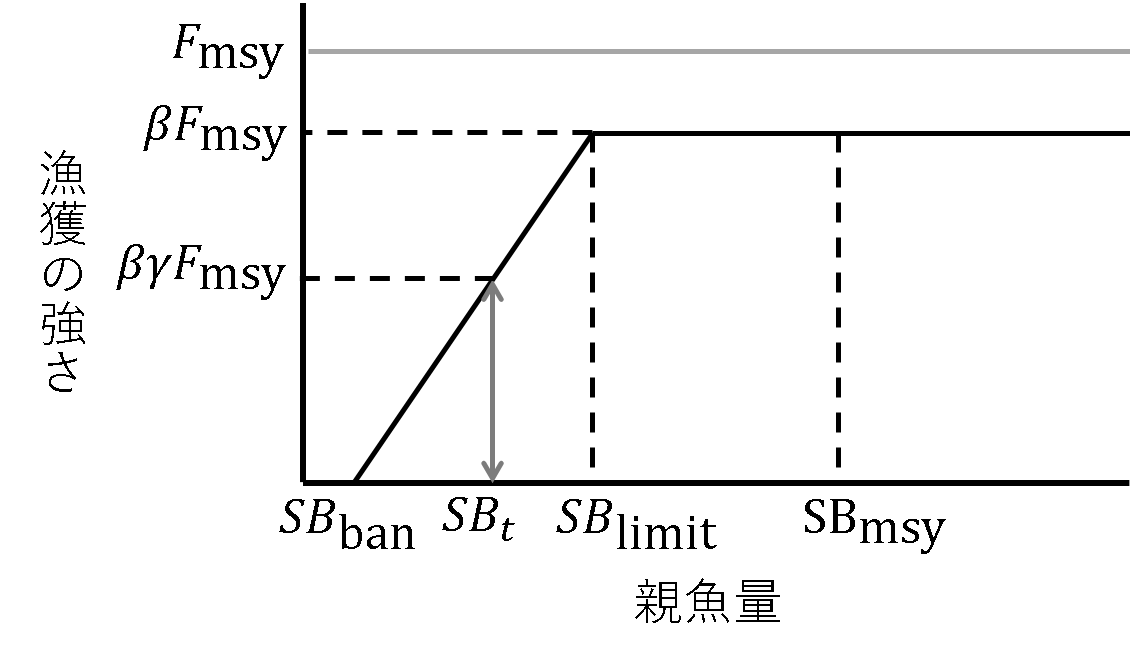
\includegraphics[width=5cm]{fig_HCR.png}  
  \caption{
    1系資源の漁獲制御ルールの模式図
  }
  \label{fig_HCR}
\end{figure}

\section{その他}
\subsection{再生産関係の誤りによるABCの推定誤差を考慮した簡易MSE\label{sec:mse}}

ABCは式\label{ABC_eq1} 式\label{ABC_eq2}により、資源評価最終年$T_3$年の2年後$T_3+2$年の漁獲量の平均値として与えられる。この値は、(資源評価の誤差がないと仮定すると)既知である$T_3$年までの資源状態から、$T_3+1$年と$T_3+2$年分将来予測実施した結果を利用している。したがってABCを計算するさいには、$T_3+1$年と$T_3+2$年の加入尾数・年齢別体重・自然死亡係数・成熟率、また、$T_3+1$年の年齢別漁獲係数、さらに、HCRを用いて漁獲量を計算する$T_3+2$年にはHCRのパラメータとして$S\!B_{\mathrm{limit}}$・$S\!B_{\mathrm{ban}}$・$F_{\mathrm{msy},s}$が必要となる。

資源評価の誤差がない理想的な条件においても、再生産関係を一つに決定するための十分な情報が得られない場合がある。また、選択した再生産関係とは異なる再生産関係がもし真であった場合、バイアスのある再生産関係から管理基準値やABCがバイアスする恐れがある。そこで、再生産関係の選択のミスから生じる管理基準値やABCのリスクを評価するため、再生産関係の選択のミスがあるような状況を想定したシミュレーションを実施する。

資源量推定や管理誤差の不確実性を考慮したシミュレーションは一般に管理戦略評価(Management Strategy Evaluation, MSE)と呼ばれているが(引用)、本シミュレーションでは不確実性を考慮する範囲が狭いため、あくまで簡易的なMSEである。本MSEで正しいと仮定する数値と考慮する不確実性を以下にまとめた。ここでは、将来予測の任意の年$T_6$年における漁獲量を決定する場合である。
\begin{itemize}
\item 正しく知っているとするもの:$T_6-1$年と$T_6$年の年齢別体重・自然死亡係数・成熟率、$T_6-1$年の年齢別漁獲係数
\item 間違った再生産関係を用いた場合に間違う値:$T_6-1$年と$T_6$年の加入尾数($N_{S_{\mathrm{min}},T_6 -1}, N_{S_{\mathrm{min}},T_6}$)、$S\!B_{\mathrm{limit}}$・$S\!B_{\mathrm{ban}}$(つまり$\gamma$)・$F_{\mathrm{msy},s}$、ひいては$T_6-1$年ABC($ABC_{T_6-1}$)。真の値に対して、将来予測による推定値を$N_{S_{\mathrm{min}},T_6-1}', N_{S_{\mathrm{min}},T_6}'$)、$S\!B_{\mathrm{limit}}'$・$S\!B_{\mathrm{ban}}'$・$F_{\mathrm{msy},s}'$・$\gamma'$・$ABC_{T_6}'$とする。
\end{itemize}

シミュレーションでは上記の方法によって推定されたABC($ABC_{T_6}'$)が$T_6$年のTACとして与えられ、$ABC_{T_6}'$どおりの漁獲が行われるとする。つまり、$T_6$年の漁獲量は
\begin{eqnarray}
  {C'}_{T_6}^{k}={ABC'}_{T_6}^{k}=\sum_{s=S_{\mathrm{min}}}^{S_{\mathrm{max}}} \frac{{F'}_{s,T_6}^k}{{F'}_{s,T_6}^k+M_{s,T_6}}
  \exp(- {F'}_{s,T_6}^k - M_{s,T_6}) N_{s,T_6}^k v_{s,T_6}
\label{ABC_eq1}
\end{eqnarray}
Popeの近似式を使っている場合には
\begin{eqnarray}
  {C'}_{T_6}^k={ABC'}_{T_6}^{k}=\sum_{s=S_{\mathrm{min}}}^{S_{\mathrm{max}}} (1-\exp(- {F'}_{s,T_6}^k)) \exp(-\frac{M_{s,T_6}}{2}) N_{s,T_6}^k v_{s,T_6}
\label{ABC_eq2}
\end{eqnarray}
となる。ここで、${F'}_{s,T_6}^k$は、右辺と左辺が一致するような$c \beta \gamma' F_{\mathrm{msy},s}$な定数$c$を探索的に求め、そのときの漁獲係数($c \beta \gamma F_{\mathrm{msy},s}$)に相当する。真の個体群動態は式\label{future_eq3}の$F_{s,T_6}^k$を${F'}_{s,T_6}^k$で置き換えたものを用いる。

ここで、簡易MSEの中でABC計算のさいに推定された加入尾数やABCの相対誤差(Relative error)を評価するため、以下のような相対誤差の指標を計算する。加入尾数の推定誤差は
\begin{eqnarray}
  R\!E_{\mathrm{rec}} = \frac{(R_{T_6}-R'_{T_6})}{R_{T_6}}
\label{RE1}
\end{eqnarray}
とした。また、ABCの相対誤差は
\begin{eqnarray}
  R\!E_{\mathrm{ABC-true}} = \frac{(ABC_{T_6}-ABC'_{T_6})}{ABC_{T_6}}
\label{ABC_eq1}
\end{eqnarray}
と
\begin{eqnarray}
  R\!E_{\mathrm{ABC-pseudo}} = \frac{(ABC_{T_6, pseudo}-ABC'_{T_6})}{ABC_{T_6}}
\label{ABC_eq2}
\end{eqnarray}
の2通りを計算した。$ABC_{T_6}$は全てのパラメータを真の値で計算したときのABC、$ABC_{T_6, pseudo}$はABC計算のさいに$T_6-1$年と$T_6$年の加入尾数($N_{S_{\mathrm{min}},T_6 -1}, N_{S_{\mathrm{min}},T_6}$)だけ真の値を用いて計算したABC(管理基準値のみ間違っている)である。簡易MSEの適用例と結果の解釈については市野川 (2020, FRA-SA2020-BRP01-07)で詳述している。

\subsection{過去にさかのぼって管理をおこなった場合のシミュレーション\label{sec:whatif}}

過去に実際に見られた加入のパターンのもとで、もしMSY管理基準値に基づいたHCRに従って漁獲を調整していたら過去の資源量はどのように変化していたかをシミュレーションする。本シミュレーションでは、過去の任意の年($T_5$年)の年齢別資源尾数$N_{s,T_5}$から資源評価最終年$T_3$まで、式\ref{future_eq3}に従った前進計算をおこなう。そのさいの生物パラメータ($M_{s,t}$、$m_{s,t}$、$w_{s,t}$、$v_{s,t}$)は過去に見られた実際の値(VPAへの入力値)を用いる。$T_5 \leq t \leq T_3$の期間の漁獲係数$F_{s,t}$は、式\ref{future_eq4}における$t > T_3+1$の場合の条件の場合の式を用いる。これはつまり、$T_5$年からHCRに従って漁獲係数を調整した場合を想定している。

$T_5+1$年からは、過去の再生産関係から推定された再生産関数とパラメータ($\mathrm{R}(S\!B_{T}^k|a,b)$)を期待値とした加入が発生すると考える。毎年の加入の残差は、過去に見られた残差をそのまま使った場合(シナリオ1)に加えて、残差を確率分布で発生させる場合(シナリオ2)も計算した。シナリオ1もシナリオ2も、HCRを用いて漁獲係数を調整したことにより、親魚量が過去に実現されたものとは異なってくるため、過去の加入尾数の期待値も変化する。シナリオ1では、実際の加入尾数の期待値からの確率的なずれを、(環境の良し悪しには漁獲のコントロールが影響しないと考えて)過去に見られた残差の値をそのまま用いる。シナリオ2では、対数残差が正規分布に従うと考えて確率的に値を発生させるシミュレーションを繰り返す($t$年($T_5 \leq t \leq T_3$)の時点で、将来の生物パラメータを既知として将来予測を実施することに相当する)。シナリオ1の結果は、シナリオ2のうちの一つの実現値にあたる。

\begin{itemize}
\item 1. \ref{SRest}節で推定された再生産関係のパラメータ$a$,$b$,$rho$に従って過去の$T$年($T_5 \leq t \leq T_3$)の加入尾数の期待値 $\mathrm{R}(S\!B_{T}|a,b)$を計算し、その予測値に過去に実現された加入尾数の残差$\varepsilon_{T}$を指数変換したものを乗じる($ N_{S_{\mathrm{min}},t} = \mathrm{R}(S\!B_{t}|a,b) \exp (\varepsilon_T)$)。
\item 2. $T$年の加入尾数の期待値シナリオ1と同じ方法で計算するが、加入の残差は$\varepsilon_{T}^k \sim \mathrm{Normal} (\rho \varepsilon_{T-1}^k,(1-\rho^2) \sigma^2)$とする。
\end{itemize}

また、マイワシ対馬暖流系群のように、年によって再生産関係のパラメータが異なると仮定されている場合、本シミュレーションで仮定される過去の再生産関係は、パラメータ推定のさいに仮定した同じ年に再生産関係が切り替わるとしている。図\ref{fig_whatif}は対馬暖流系群で過去にさかのぼったシミュレーションを実施したときの例。

 \begin{figure}[b]
   \includegraphics[keepaspectratio, scale=0.17]{figs/g1_withCI.jpg}
   \caption{
     マイワシ対馬暖流系群で過去にさかのぼった場合のシミュレーションを実施した例。1990年(start\_from1990)、2000年(start\_from2000)、2005年(start\_from2005)から、通常レジームの管理基準値を使って管理を開始した3通りの結果の比較。細い実線は過去に見られた残差をそのまま用いたもの(シナリオ1)、塗りの範囲は過去の残差を確率分布からランダムに発生させたシミュレーションの90%信頼区間、太い実線はシミュレーションの結果の平均値。親魚量が禁漁水準を割っている2000年、2005年では、管理開始当初の漁獲量はゼロになったのち、親魚量が回復したのちに漁獲が再開している。
   }
   \label{fig_whatif}
 \end{figure}

% \subsection{平均された再生産関係を用いた管理基準値の計算}
 
% \subsection{年齢別体重における密度依存的な変化について}


\begin{thebibliography}{9}
  \bibitem{hockey} Clark CW, Charles AT, Beddington JR, Mangel M (1985) Optimal capacity decisions in a developing fishery. Marine Resource Economics 2:25--53.
\bibitem{beverton} Beverton RJH, Holt SJ (1957) On the Dynamics of Exploited Fish Populations. Her Majesty’s Stationary Office, London.
\bibitem{ricker} Ricker WE (1954) Stock and recruitment. Journal of Fisheries Research Board of Canada 11:559--623.
\bibitem{thorson} Thorson JT, Jensen OP, Zipkinc EF (2014) How variable is recruitment for exploited marine fishes? Can J Fish Aquat Sci 71:973--983
\bibitem{johnson} Johnson KF, Council E, Thorson JT, Brooks E, Methot RD, Punt AE (2016) Can autocorrelated recruitment be estimated using integrated assessment models and how does it affect population forecasts? Fish Res 183:222--232
\bibitem{R} R Core Team (2018) R: A language and environment for statistical computing. R Foundation for Statistical Computing, Vienna, Austria. https://www.R-project.org/
\bibitem{rho_simulation} FRA-SA2020-BRP01-06. 市野川桃子, 西嶋翔太, 岡村 寛 (2020) シミュレーションを用いた自己相関係数の同時推定手法の推定バイアス評価.
\bibitem{mse_simulation} FRA-SA2020-BRP01-07. 市野川桃子 (2020) 簡易的MSEを用いた複数の管理基準値の頑健静の比較・HCRの検討.
  
%\bibitem{ichinokawa} 市野川桃子・岡村 寛 (2014) VPAを用いた我が国水産資源評価の統計言語Rによる統一的検討. 水産海洋研究 78:104--113

\end{thebibliography}

\begin{table}[h]
  \caption{本資料で用いられる数式の記号の定義}  
  \begin{tabular}{cp{11cm}} \hline
    記号    &  説明 \\ \hline
    $t$ & 時間 (time) の次元を表す添え字.通常は年なので,ここでは$t$年といった表記を使用する.資源評価開始年を$t=1$, 資源評価最終年を$t=T_3$とする.将来予測開始年は$t=T_{3}+1$,一定の漁獲圧で漁獲して平衡状態に達したときの年を$T_4$とする.また,再生産関係の推定のためにデータを用いる最初の加入年を$T_1$,最後の加入年を$T_2$とする.通常は,$1 \leq T_1 < T_2 \leq T_3 \ll T_4$.\\
    $s$ & 成長段階 (stage) を表す添え字.通常は年齢なので,ここでは$s$歳といった表記を使用する.$s=S_{\mathrm{min}},...,S_{\mathrm{max}}$で,$S_{\mathrm{min}}$は加入年齢,$S_{\mathrm{max}}$は$S_{\mathrm{max}}$歳以上をひとまとめにしたグループ(プラスグループ).\\ % 次年度版はaにする
    $N_{s,t}$ & $s$歳$t$年の資源尾数.たとえば加入尾数は$N_{s_{\mathrm{min}},t}$となる.\\
    $F_{s,t}$ & $s$歳$t$年における漁獲死亡係数\\
    $M_{s,t}$ & $s$歳$t$年における自然死亡係数\\
    $m_{s,t}$ & $s$歳$t$年における成熟率\\
    $w_{s,t}$ & 親魚量を計算するときの$s$歳$t$年の個体あたりの体重\\
    $v_{s,t}$ & 漁獲量を計算するときの$s$歳$t$年の個体あたりの体重\\ % 資源量を計算するときの体重も追記する?当面は必要ないが,次回は追記するかも.
    $S\!B_{t} $ & $t$年の親魚資源量.$S\!B_t=\sum_{s=S\mathrm{min}}^{S_{\mathrm{max}}}N_{s,t} w_{s,t} m_{s,t}$.\\
    $B_{t} $ & $t$年の総資源量.$\!B_t=\sum_{s=S\mathrm{min}}^{S_{\mathrm{max}}}N_{s,t} w_{s,t}$.\\    
    $k$      & 確率的な将来予測シミュレーションにおける各試行に対する添字.将来予測の期間で各パラメータの右上につけて各試行ごとの値を示す.例えば,将来予測における加入尾数の場合は$N_{S_{\mathrm{min}},t}^k$, 親魚量の場合は$S\!B_t^k$のように使用する.$k=1,…,K$.\\
    $\mathrm{obs}$  & 資源評価モデルにより得られた過去の資源評価値に対する添字.再生産関係を推定する際には観測値(observation)として取り扱うため,$\mathrm{obs}$と表記した.例えば過去の加入尾数は$N_{s_{\mathrm{min}},t}^{\mathrm{obs}}$となる.\\
    $G$       & 世代時間(年).$\sum_{s=0}^\infty (s \exp(-\sum_s M_{s,t}) m_{s,t})/(\exp(-\sum_s M_{s,t}) m_{s,t})$ と定義する.\\ % Rの関数では加入年齢からになっていた.次バージョンでは0歳から計算するように修正すること\\
    $n$ & 再生産関係推定に用いるデータの数.$n=T_2-T_1+1$.\\    
    $\varepsilon_t$  & $t$年の再生産関係からの加入尾数の予測値と観測値の対数残差\\
    $\sigma$  & 再生産関係からの加入尾数の予測値と観測値の対数残差における標準偏差\\
    $\rho$  & 加入の対数値の残差の自己相関係数\\
    $\kappa$  & 将来予測における加入尾数のバイアス補正のための係数\\    
    $a$, $b$  & 再生産関係で推定されるパラメータ \\  %.$a$は最大増加率,$b$は密度効果の大きさを示す.\\  \hline% 次期バージョンではh, R0を表に出すパラメータとする.HSにおけるsteepnessは1-B_HS/B_0と定義
    $\mathrm{R}(S\!B_{t}|a,b)$ &  パラメータa,bと親魚資源量$S\!B_{t}$を持つ再生産関係式,またはそこから計算される加入尾数の期待値 \\   \hline
  \end{tabular}
  \label{table_definition} 
\end{table}

\end{document}


